\documentclass[9pt]{exam} 
\addpoints
\pointsinmargin

\usepackage[fleqn]{amsmath}
\usepackage{amssymb} %standard classy maths symbols
\usepackage[a4paper, margin=1in]{geometry} %makes it easy to specify where to put stuff on the page

\usepackage{tcolorbox} % basic but good package for boxes around text
\tcbset{colback=black!5!white}

\usepackage{tikz} % interval diagrams, sets, etc.

\begin{document}

\textbf{Name:} \dotfill

\

Take $E_1(1, 0)$ on the $x$-axis and $E_2(0, 1)$ on the $y$-axis of an orthonormal coordinate system on the plane with origin $O$. Define $\overrightarrow{e_1} = \overrightarrow{OE_1}$ and $\overrightarrow{e_2} = \overrightarrow{OE_2}$. Then for any point $A$ in the plane we have
$$ A(a_1, a_2) \quad \iff \quad \overrightarrow{OA} = a_1 \cdot \overrightarrow{e_1} + a_2 \cdot \overrightarrow{e_2} = \left( \begin{matrix} a_1 \\ a_2 \end{matrix} \right). \qquad \mbox{This last expression is called \emph{column notation}}.$$

\vspace{-8mm}

\begin{center}
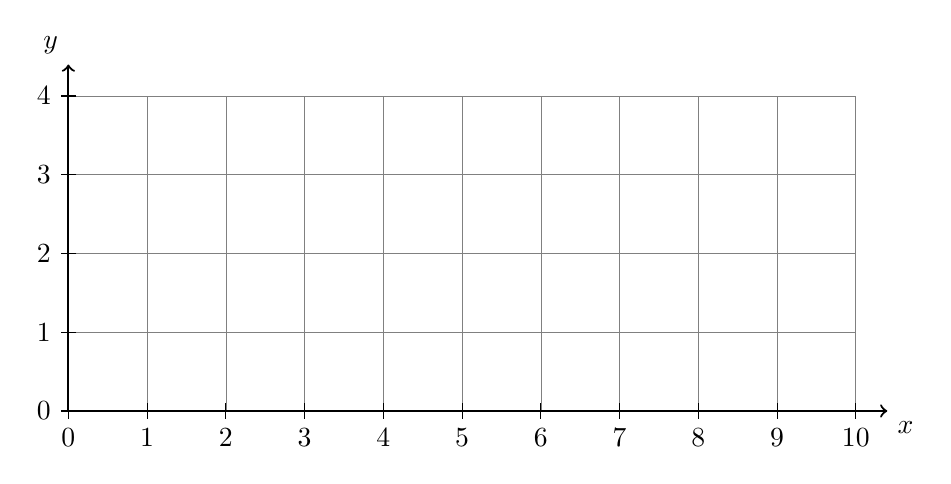
\begin{tikzpicture}

% Draw the grid
\draw[step=1cm,gray,very thin] (0,0) grid (10,4);

% Draw the x-axis
\draw[thick,->] (0,0) -- (10.4,0) node[anchor=north west] {$x$};

% Draw the y-axis
\draw[thick,->] (0,0) -- (0,4.4) node[anchor=south east] {$y$};

% Labels for the axes
\foreach \x in {0,1,...,10} \draw (\x,0.1) -- (\x,-0.1) node[anchor=north] {\x};
\foreach \y in {0,1,...,4} \draw (0.1,\y) -- (-0.1,\y) node[anchor=east] {\y};

\end{tikzpicture}
\end{center}



\begin{questions} 
\question[4] Mark the arrows $\overrightarrow{e_1}$, $\overrightarrow{e_2}$, $\overrightarrow{OX}$, and $\overrightarrow{OY}$ on the plane above, for $X(6, 3)$ and $Y(2, 4)$.

\question[4] Rewrite and simplify the following vectors using column notation :

\

\begin{parts}
\part $\overrightarrow{OX}$ = \dotfill

\

\part $\overrightarrow{XY}$ = \dotfill

\

\part $\overrightarrow{YX} + 2 \overrightarrow{YO}$ = \dotfill
\fillwithdottedlines{12mm}
\end{parts}

\question[3] For the general point $A(a_1, a_2)$, derive $\| \overrightarrow{a} \|$ in terms of $a_1, a_2$ using Pythagoras. \hfill \emph{Check hypotheses!}
\fillwithdottedlines{5cm}


\vfill

\question[0] \textbf{Bonus.} 
Let $\overrightarrow{a} = 5 \cdot \overrightarrow{e_1} + \overrightarrow{e_2}$ and $\overrightarrow{b} = \lambda \cdot \overrightarrow{e_1} + 3 \cdot \overrightarrow{e_2}$. \newline
Given that $\|3 \cdot \overrightarrow{a} + \overrightarrow{b}\| = 10$ find the possible values of $\lambda$.
\hfill \emph{Work on the back.}

\end{questions}


\begin{tcolorbox}

\textbf{Name of marker:}

\begin{center}
\gradetable[h][questions]
\end{center}

\end{tcolorbox}


\end{document}